\section{Learning Objectives}

After completing this chapter, readers will be able to:
\begin{itemize}
    \item Understand fundamental distributed training strategies and when to apply them
    \item Implement data parallelism using PyTorch Distributed Data Parallel (DDP)
    \item Design and implement model parallelism for models that don't fit on single GPUs
    \item Choose between parameter server and all-reduce architectures
    \item Implement synchronous and asynchronous gradient synchronization
    \item Build fault-tolerant distributed training systems with checkpointing
    \item Optimize resource allocation and scheduling for multi-node training
    \item Use Horovod for framework-agnostic distributed training
    \item Apply Ray for flexible distributed computing workflows
    \item Benchmark and optimize distributed training performance
    \item Identify and resolve common bottlenecks in distributed systems
\end{itemize}

\section{Introduction: Why Distributed Training?}

Modern deep learning models and datasets have grown beyond the capacity of single GPUs. Consider:

\begin{itemize}
    \item \textbf{Model Size}: GPT-3 has 175 billion parameters requiring ~700GB memory
    \item \textbf{Dataset Scale}: ImageNet-21k contains 14 million images
    \item \textbf{Training Time}: Training BERT from scratch takes weeks on single GPU
    \item \textbf{Research Velocity}: Faster iteration enables more experiments
\end{itemize}

Distributed training addresses these challenges through parallelization across multiple devices, but introduces new complexities:

\begin{itemize}
    \item Communication overhead between devices
    \item Gradient synchronization strategies
    \item Fault tolerance and recovery
    \item Resource allocation and scheduling
    \item Debugging and monitoring across nodes
\end{itemize}

\subsection{Scaling Laws}

Understanding scaling efficiency is crucial for distributed training:

\begin{equation}
\text{Speedup} = \frac{T_1}{T_N}
\end{equation}

where $T_1$ is training time on 1 GPU and $T_N$ is training time on $N$ GPUs.

\begin{equation}
\text{Scaling Efficiency} = \frac{\text{Speedup}}{N} = \frac{T_1}{N \cdot T_N}
\end{equation}

Perfect linear scaling achieves efficiency = 1.0, but communication overhead typically reduces this to 0.7-0.9 in practice.

\section{Data Parallelism}

Data parallelism replicates the model across devices and distributes data batches. Each device computes gradients on its batch, then gradients are synchronized.

\begin{figure}[h]
\centering
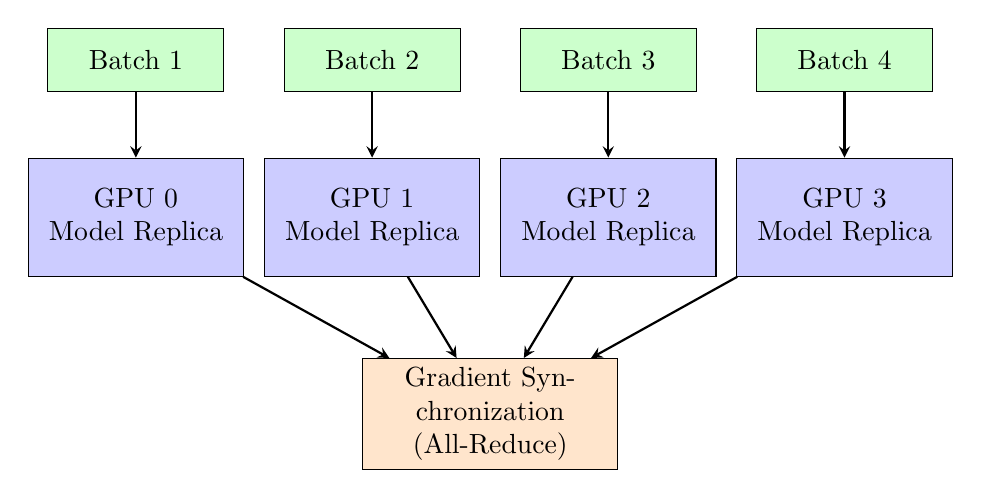
\begin{tikzpicture}[node distance=2.5cm, auto]
    \tikzstyle{gpu} = [rectangle, draw, fill=blue!20, text width=2.5cm, text centered, minimum height=1.5cm]
    \tikzstyle{data} = [rectangle, draw, fill=green!20, text width=2cm, text centered, minimum height=0.8cm]
    \tikzstyle{sync} = [rectangle, draw, fill=orange!20, text width=3cm, text centered, minimum height=0.8cm]
    \tikzstyle{arrow} = [thick,->,>=stealth]

    % Data batches
    \node [data] (batch1) {Batch 1};
    \node [data, right of=batch1, node distance=3cm] (batch2) {Batch 2};
    \node [data, right of=batch2, node distance=3cm] (batch3) {Batch 3};
    \node [data, right of=batch3, node distance=3cm] (batch4) {Batch 4};

    % GPUs
    \node [gpu, below of=batch1, node distance=2cm] (gpu1) {GPU 0\\Model Replica};
    \node [gpu, below of=batch2, node distance=2cm] (gpu2) {GPU 1\\Model Replica};
    \node [gpu, below of=batch3, node distance=2cm] (gpu3) {GPU 2\\Model Replica};
    \node [gpu, below of=batch4, node distance=2cm] (gpu4) {GPU 3\\Model Replica};

    % Sync
    \node [sync, below of=gpu2, node distance=2.5cm, xshift=1.5cm] (sync) {Gradient Synchronization\\(All-Reduce)};

    \draw [arrow] (batch1) -- (gpu1);
    \draw [arrow] (batch2) -- (gpu2);
    \draw [arrow] (batch3) -- (gpu3);
    \draw [arrow] (batch4) -- (gpu4);

    \draw [arrow] (gpu1) -- (sync);
    \draw [arrow] (gpu2) -- (sync);
    \draw [arrow] (gpu3) -- (sync);
    \draw [arrow] (gpu4) -- (sync);
\end{tikzpicture}
\caption{Data parallelism: Model replicated across GPUs, data distributed}
\label{fig:data_parallelism}
\end{figure}

\subsection{PyTorch Distributed Data Parallel (DDP)}

PyTorch DDP provides efficient data parallelism with optimized gradient synchronization.

\begin{lstlisting}[style=python, caption=Complete PyTorch DDP implementation]
import torch
import torch.nn as nn
import torch.distributed as dist
import torch.multiprocessing as mp
from torch.nn.parallel import DistributedDataParallel as DDP
from torch.utils.data import DataLoader, DistributedSampler
import os
import argparse

class ResNetModel(nn.Module):
    """Example model for distributed training"""
    def __init__(self, num_classes=10):
        super().__init__()
        self.conv1 = nn.Conv2d(3, 64, kernel_size=7, stride=2, padding=3)
        self.bn1 = nn.BatchNorm2d(64)
        self.relu = nn.ReLU(inplace=True)
        self.maxpool = nn.MaxPool2d(kernel_size=3, stride=2, padding=1)

        # Residual blocks
        self.layer1 = self._make_layer(64, 128, 3)
        self.layer2 = self._make_layer(128, 256, 4)
        self.layer3 = self._make_layer(256, 512, 6)

        self.avgpool = nn.AdaptiveAvgPool2d((1, 1))
        self.fc = nn.Linear(512, num_classes)

    def _make_layer(self, in_channels, out_channels, num_blocks):
        layers = []
        layers.append(nn.Conv2d(in_channels, out_channels, 3, stride=2, padding=1))
        layers.append(nn.BatchNorm2d(out_channels))
        layers.append(nn.ReLU(inplace=True))

        for _ in range(num_blocks - 1):
            layers.append(nn.Conv2d(out_channels, out_channels, 3, padding=1))
            layers.append(nn.BatchNorm2d(out_channels))
            layers.append(nn.ReLU(inplace=True))

        return nn.Sequential(*layers)

    def forward(self, x):
        x = self.conv1(x)
        x = self.bn1(x)
        x = self.relu(x)
        x = self.maxpool(x)

        x = self.layer1(x)
        x = self.layer2(x)
        x = self.layer3(x)

        x = self.avgpool(x)
        x = torch.flatten(x, 1)
        x = self.fc(x)
        return x

def setup_distributed(rank, world_size, backend='nccl'):
    """Initialize distributed training process group"""
    os.environ['MASTER_ADDR'] = 'localhost'
    os.environ['MASTER_PORT'] = '12355'

    # Initialize process group
    dist.init_process_group(
        backend=backend,
        rank=rank,
        world_size=world_size
    )

    # Set device
    torch.cuda.set_device(rank)

def cleanup_distributed():
    """Clean up distributed training"""
    dist.destroy_process_group()

def create_dataloader(rank, world_size, batch_size):
    """Create distributed dataloader"""
    from torchvision import datasets, transforms

    # Data transformations
    transform = transforms.Compose([
        transforms.RandomResizedCrop(224),
        transforms.RandomHorizontalFlip(),
        transforms.ToTensor(),
        transforms.Normalize(mean=[0.485, 0.456, 0.406],
                           std=[0.229, 0.224, 0.225])
    ])

    # Dataset
    dataset = datasets.FakeData(
        size=10000,
        image_size=(3, 224, 224),
        num_classes=10,
        transform=transform
    )

    # Distributed sampler ensures each GPU gets different data
    sampler = DistributedSampler(
        dataset,
        num_replicas=world_size,
        rank=rank,
        shuffle=True,
        drop_last=True
    )

    # DataLoader
    loader = DataLoader(
        dataset,
        batch_size=batch_size,
        sampler=sampler,
        num_workers=4,
        pin_memory=True,
        persistent_workers=True
    )

    return loader, sampler

def train_epoch(model, dataloader, criterion, optimizer, rank, epoch):
    """Train for one epoch"""
    model.train()
    total_loss = 0.0
    correct = 0
    total = 0

    for batch_idx, (data, target) in enumerate(dataloader):
        # Move to GPU
        data = data.cuda(rank, non_blocking=True)
        target = target.cuda(rank, non_blocking=True)

        # Forward pass
        optimizer.zero_grad(set_to_none=True)  # More efficient than zero_grad()
        output = model(data)
        loss = criterion(output, target)

        # Backward pass
        loss.backward()

        # Gradient clipping (optional but recommended)
        torch.nn.utils.clip_grad_norm_(model.parameters(), max_norm=1.0)

        # Optimizer step
        optimizer.step()

        # Statistics
        total_loss += loss.item()
        _, predicted = output.max(1)
        total += target.size(0)
        correct += predicted.eq(target).sum().item()

        if rank == 0 and batch_idx % 10 == 0:
            print(f'Epoch: {epoch} | Batch: {batch_idx}/{len(dataloader)} | '
                  f'Loss: {loss.item():.4f} | '
                  f'Acc: {100.*correct/total:.2f}%')

    # Gather statistics from all processes
    avg_loss = total_loss / len(dataloader)
    accuracy = 100. * correct / total

    return avg_loss, accuracy

def validate(model, dataloader, criterion, rank):
    """Validate model"""
    model.eval()
    total_loss = 0.0
    correct = 0
    total = 0

    with torch.no_grad():
        for data, target in dataloader:
            data = data.cuda(rank, non_blocking=True)
            target = target.cuda(rank, non_blocking=True)

            output = model(data)
            loss = criterion(output, target)

            total_loss += loss.item()
            _, predicted = output.max(1)
            total += target.size(0)
            correct += predicted.eq(target).sum().item()

    avg_loss = total_loss / len(dataloader)
    accuracy = 100. * correct / total

    # Synchronize metrics across all GPUs
    loss_tensor = torch.tensor(avg_loss).cuda(rank)
    acc_tensor = torch.tensor(accuracy).cuda(rank)

    dist.all_reduce(loss_tensor, op=dist.ReduceOp.SUM)
    dist.all_reduce(acc_tensor, op=dist.ReduceOp.SUM)

    world_size = dist.get_world_size()
    avg_loss = loss_tensor.item() / world_size
    accuracy = acc_tensor.item() / world_size

    return avg_loss, accuracy

def save_checkpoint(model, optimizer, epoch, loss, filepath, rank):
    """Save checkpoint (only rank 0)"""
    if rank == 0:
        checkpoint = {
            'epoch': epoch,
            'model_state_dict': model.module.state_dict(),  # .module for DDP
            'optimizer_state_dict': optimizer.state_dict(),
            'loss': loss,
        }
        torch.save(checkpoint, filepath)
        print(f'Checkpoint saved: {filepath}')

def load_checkpoint(filepath, model, optimizer=None):
    """Load checkpoint"""
    checkpoint = torch.load(filepath)
    model.module.load_state_dict(checkpoint['model_state_dict'])
    if optimizer:
        optimizer.load_state_dict(checkpoint['optimizer_state_dict'])
    return checkpoint['epoch'], checkpoint['loss']

def train_ddp(rank, world_size, args):
    """Main distributed training function"""
    print(f'Running DDP on rank {rank}')

    # Setup
    setup_distributed(rank, world_size)

    # Create model and move to GPU
    model = ResNetModel(num_classes=args.num_classes).cuda(rank)

    # Wrap model with DDP
    model = DDP(
        model,
        device_ids=[rank],
        output_device=rank,
        find_unused_parameters=False,  # Set True only if needed
        gradient_as_bucket_view=True   # Memory optimization
    )

    # Loss and optimizer
    criterion = nn.CrossEntropyLoss().cuda(rank)
    optimizer = torch.optim.SGD(
        model.parameters(),
        lr=args.lr,
        momentum=0.9,
        weight_decay=1e-4
    )

    # Learning rate scheduler
    scheduler = torch.optim.lr_scheduler.CosineAnnealingLR(
        optimizer,
        T_max=args.epochs
    )

    # Create dataloaders
    train_loader, train_sampler = create_dataloader(
        rank, world_size, args.batch_size
    )
    val_loader, _ = create_dataloader(
        rank, world_size, args.batch_size
    )

    # Training loop
    best_acc = 0.0
    start_epoch = 0

    # Resume from checkpoint if exists
    if args.resume and os.path.exists(args.resume):
        start_epoch, _ = load_checkpoint(args.resume, model, optimizer)
        print(f'Resumed from epoch {start_epoch}')

    for epoch in range(start_epoch, args.epochs):
        # Set epoch for distributed sampler (important for shuffling)
        train_sampler.set_epoch(epoch)

        # Train
        train_loss, train_acc = train_epoch(
            model, train_loader, criterion, optimizer, rank, epoch
        )

        # Validate
        val_loss, val_acc = validate(model, val_loader, criterion, rank)

        # Update learning rate
        scheduler.step()

        # Print stats (rank 0 only)
        if rank == 0:
            print(f'\nEpoch {epoch}:')
            print(f'  Train Loss: {train_loss:.4f} | Train Acc: {train_acc:.2f}%')
            print(f'  Val Loss: {val_loss:.4f} | Val Acc: {val_acc:.2f}%')
            print(f'  LR: {scheduler.get_last_lr()[0]:.6f}\n')

        # Save checkpoint
        if val_acc > best_acc:
            best_acc = val_acc
            save_checkpoint(
                model, optimizer, epoch, val_loss,
                f'checkpoint_best.pth', rank
            )

        # Regular checkpoint
        if (epoch + 1) % args.save_freq == 0:
            save_checkpoint(
                model, optimizer, epoch, val_loss,
                f'checkpoint_epoch_{epoch}.pth', rank
            )

    # Cleanup
    cleanup_distributed()

def main():
    parser = argparse.ArgumentParser(description='PyTorch DDP Training')
    parser.add_argument('--epochs', type=int, default=100)
    parser.add_argument('--batch-size', type=int, default=64)
    parser.add_argument('--lr', type=float, default=0.1)
    parser.add_argument('--num-classes', type=int, default=10)
    parser.add_argument('--resume', type=str, default=None)
    parser.add_argument('--save-freq', type=int, default=10)
    args = parser.parse_args()

    # World size = number of GPUs
    world_size = torch.cuda.device_count()
    print(f'Training on {world_size} GPUs')

    # Spawn processes for each GPU
    mp.spawn(
        train_ddp,
        args=(world_size, args),
        nprocs=world_size,
        join=True
    )

if __name__ == '__main__':
    main()
\end{lstlisting}

\subsection{Launch Script for Multi-Node Training}

For multi-node training, use \texttt{torchrun} (formerly \texttt{torch.distributed.launch}):

\begin{lstlisting}[style=shell, caption=Multi-node DDP training script]
#!/bin/bash
# Launch on each node

# Node 0 (master)
torchrun \
    --nproc_per_node=4 \
    --nnodes=2 \
    --node_rank=0 \
    --master_addr="192.168.1.1" \
    --master_port=12355 \
    train_ddp.py \
    --epochs 100 \
    --batch-size 64

# Node 1
torchrun \
    --nproc_per_node=4 \
    --nnodes=2 \
    --node_rank=1 \
    --master_addr="192.168.1.1" \
    --master_port=12355 \
    train_ddp.py \
    --epochs 100 \
    --batch-size 64
\end{lstlisting}

\section{Model Parallelism}

Model parallelism splits the model across devices when it's too large to fit on a single GPU. Different parts of the model reside on different GPUs.

\begin{figure}[h]
\centering
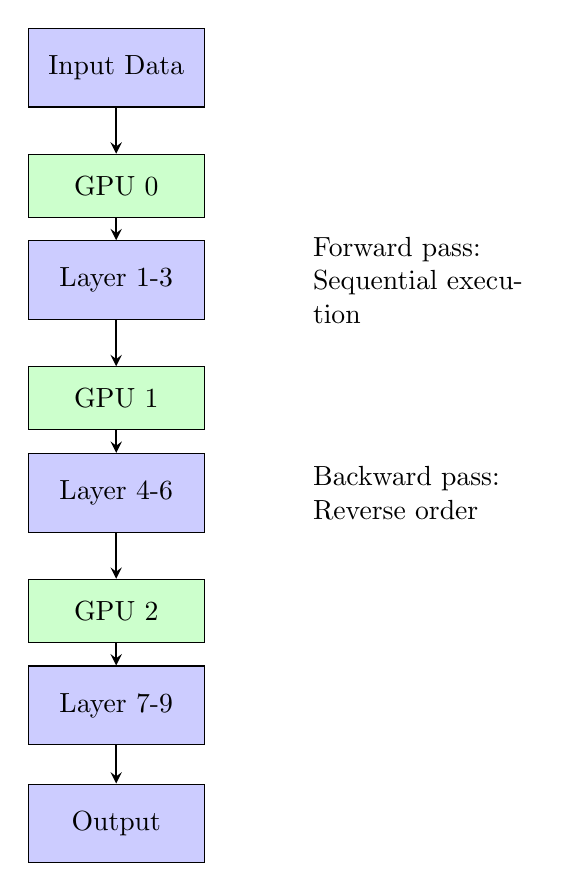
\begin{tikzpicture}[node distance=2.5cm, auto]
    \tikzstyle{layer} = [rectangle, draw, fill=blue!20, text width=2cm, text centered, minimum height=1cm]
    \tikzstyle{gpu} = [rectangle, draw, fill=green!20, text width=2cm, text centered, minimum height=0.8cm]
    \tikzstyle{arrow} = [thick,->,>=stealth]

    % Input
    \node [layer] (input) {Input Data};

    % GPU 0 layers
    \node [gpu, below of=input, node distance=1.5cm] (gpu0) {GPU 0};
    \node [layer, below of=gpu0, node distance=1.2cm] (layer1) {Layer 1-3};

    % GPU 1 layers
    \node [gpu, below of=layer1, node distance=1.5cm] (gpu1) {GPU 1};
    \node [layer, below of=gpu1, node distance=1.2cm] (layer2) {Layer 4-6};

    % GPU 2 layers
    \node [gpu, below of=layer2, node distance=1.5cm] (gpu2) {GPU 2};
    \node [layer, below of=gpu2, node distance=1.2cm] (layer3) {Layer 7-9};

    % Output
    \node [layer, below of=layer3, node distance=1.5cm] (output) {Output};

    \draw [arrow] (input) -- (gpu0);
    \draw [arrow] (gpu0) -- (layer1);
    \draw [arrow] (layer1) -- (gpu1);
    \draw [arrow] (gpu1) -- (layer2);
    \draw [arrow] (layer2) -- (gpu2);
    \draw [arrow] (gpu2) -- (layer3);
    \draw [arrow] (layer3) -- (output);

    \node [right of=layer1, node distance=4cm, text width=3cm] {Forward pass:\\Sequential execution};
    \node [right of=layer2, node distance=4cm, text width=3cm] {Backward pass:\\Reverse order};
\end{tikzpicture}
\caption{Model parallelism: Model layers distributed across GPUs}
\label{fig:model_parallelism}
\end{figure}

\subsection{Pipeline Parallelism}

Pipeline parallelism improves model parallelism efficiency by processing multiple micro-batches simultaneously.

\begin{lstlisting}[style=python, caption=Model parallelism with pipeline parallelism in PyTorch]
import torch
import torch.nn as nn
from torch.distributed.pipeline.sync import Pipe

class ModelParallelResNet(nn.Module):
    """ResNet with model parallelism across 2 GPUs"""
    def __init__(self, num_classes=1000):
        super().__init__()

        # Part 1: Goes to GPU 0
        self.seq1 = nn.Sequential(
            nn.Conv2d(3, 64, kernel_size=7, stride=2, padding=3),
            nn.BatchNorm2d(64),
            nn.ReLU(inplace=True),
            nn.MaxPool2d(kernel_size=3, stride=2, padding=1),
            self._make_layer(64, 128, 3),
            self._make_layer(128, 256, 4)
        ).to('cuda:0')

        # Part 2: Goes to GPU 1
        self.seq2 = nn.Sequential(
            self._make_layer(256, 512, 6),
            nn.AdaptiveAvgPool2d((1, 1)),
            nn.Flatten(),
            nn.Linear(512, num_classes)
        ).to('cuda:1')

    def _make_layer(self, in_channels, out_channels, num_blocks):
        layers = []
        layers.append(nn.Conv2d(in_channels, out_channels, 3, stride=2, padding=1))
        layers.append(nn.BatchNorm2d(out_channels))
        layers.append(nn.ReLU(inplace=True))

        for _ in range(num_blocks - 1):
            layers.append(nn.Conv2d(out_channels, out_channels, 3, padding=1))
            layers.append(nn.BatchNorm2d(out_channels))
            layers.append(nn.ReLU(inplace=True))

        return nn.Sequential(*layers)

    def forward(self, x):
        # Move input to GPU 0
        x = x.to('cuda:0')

        # Process on GPU 0
        x = self.seq1(x)

        # Transfer to GPU 1
        x = x.to('cuda:1')

        # Process on GPU 1
        x = self.seq2(x)

        return x

class PipelineParallelModel(nn.Module):
    """Model parallelism with pipeline parallelism"""
    def __init__(self, num_classes=1000, chunks=8):
        super().__init__()

        # Define model stages
        self.stage1 = nn.Sequential(
            nn.Conv2d(3, 64, kernel_size=7, stride=2, padding=3),
            nn.BatchNorm2d(64),
            nn.ReLU(inplace=True),
            nn.MaxPool2d(kernel_size=3, stride=2, padding=1),
        )

        self.stage2 = nn.Sequential(
            self._make_layer(64, 128, 3),
            self._make_layer(128, 256, 4),
        )

        self.stage3 = nn.Sequential(
            self._make_layer(256, 512, 6),
            nn.AdaptiveAvgPool2d((1, 1)),
            nn.Flatten(),
            nn.Linear(512, num_classes)
        )

        # Create pipeline
        # Each stage goes to a different GPU
        self.model = Pipe(
            nn.Sequential(self.stage1, self.stage2, self.stage3),
            chunks=chunks,  # Number of micro-batches
            checkpoint='never'  # Or 'always', 'except_last'
        )

    def _make_layer(self, in_channels, out_channels, num_blocks):
        layers = []
        layers.append(nn.Conv2d(in_channels, out_channels, 3, stride=2, padding=1))
        layers.append(nn.BatchNorm2d(out_channels))
        layers.append(nn.ReLU(inplace=True))

        for _ in range(num_blocks - 1):
            layers.append(nn.Conv2d(out_channels, out_channels, 3, padding=1))
            layers.append(nn.BatchNorm2d(out_channels))
            layers.append(nn.ReLU(inplace=True))

        return nn.Sequential(*layers)

    def forward(self, x):
        return self.model(x)

# Training with pipeline parallelism
def train_pipeline_parallel():
    model = PipelineParallelModel(num_classes=1000, chunks=8)
    criterion = nn.CrossEntropyLoss()
    optimizer = torch.optim.SGD(model.parameters(), lr=0.1)

    # Training loop
    for epoch in range(100):
        for batch_idx, (data, target) in enumerate(train_loader):
            # Pipeline handles distribution automatically
            optimizer.zero_grad()
            output = model(data)

            # Loss computation needs target on same device as output
            target = target.to(output.device)
            loss = criterion(output, target)

            loss.backward()
            optimizer.step()
\end{lstlisting}

\subsection{Tensor Parallelism}

For very large models (transformers with billions of parameters), tensor parallelism splits individual layers across GPUs.

\begin{lstlisting}[style=python, caption=Tensor parallelism for transformer layers]
import torch
import torch.nn as nn
import torch.distributed as dist

class TensorParallelLinear(nn.Module):
    """Linear layer with tensor parallelism"""
    def __init__(self, in_features, out_features, rank, world_size):
        super().__init__()
        self.rank = rank
        self.world_size = world_size

        # Each GPU holds 1/world_size of the output features
        self.out_features_per_partition = out_features // world_size

        self.weight = nn.Parameter(
            torch.randn(self.out_features_per_partition, in_features)
        )
        self.bias = nn.Parameter(
            torch.randn(self.out_features_per_partition)
        )

    def forward(self, x):
        # Local computation
        output = torch.matmul(x, self.weight.t()) + self.bias

        # All-gather outputs from all GPUs
        output_list = [torch.zeros_like(output) for _ in range(self.world_size)]
        dist.all_gather(output_list, output)

        # Concatenate outputs
        output = torch.cat(output_list, dim=-1)

        return output

class TensorParallelAttention(nn.Module):
    """Multi-head attention with tensor parallelism"""
    def __init__(self, hidden_size, num_heads, rank, world_size):
        super().__init__()
        self.hidden_size = hidden_size
        self.num_heads = num_heads
        self.rank = rank
        self.world_size = world_size

        # Ensure num_heads is divisible by world_size
        assert num_heads % world_size == 0
        self.num_heads_per_partition = num_heads // world_size

        self.head_dim = hidden_size // num_heads

        # Parallel projections
        self.q_proj = TensorParallelLinear(
            hidden_size, hidden_size, rank, world_size
        )
        self.k_proj = TensorParallelLinear(
            hidden_size, hidden_size, rank, world_size
        )
        self.v_proj = TensorParallelLinear(
            hidden_size, hidden_size, rank, world_size
        )
        self.out_proj = TensorParallelLinear(
            hidden_size, hidden_size, rank, world_size
        )

    def forward(self, x):
        batch_size, seq_len, _ = x.shape

        # Project Q, K, V (parallelized)
        q = self.q_proj(x)
        k = self.k_proj(x)
        v = self.v_proj(x)

        # Reshape for multi-head attention
        q = q.view(batch_size, seq_len, self.num_heads, self.head_dim)
        k = k.view(batch_size, seq_len, self.num_heads, self.head_dim)
        v = v.view(batch_size, seq_len, self.num_heads, self.head_dim)

        # Attention computation (local to each GPU)
        scores = torch.matmul(
            q.transpose(1, 2),
            k.transpose(1, 2).transpose(-2, -1)
        ) / (self.head_dim ** 0.5)

        attn = torch.softmax(scores, dim=-1)
        context = torch.matmul(attn, v.transpose(1, 2))

        # Reshape and project
        context = context.transpose(1, 2).contiguous()
        context = context.view(batch_size, seq_len, self.hidden_size)

        output = self.out_proj(context)

        return output
\end{lstlisting}

\section{Parameter Servers vs All-Reduce}

Two fundamental architectures for gradient synchronization in distributed training.

\subsection{Parameter Server Architecture}

Central servers store model parameters; workers fetch parameters, compute gradients, and push updates.

\begin{figure}[h]
\centering
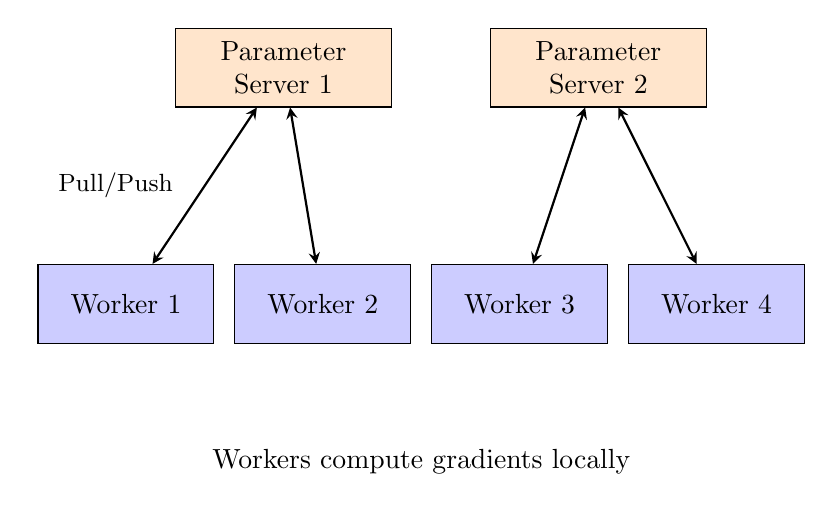
\begin{tikzpicture}[node distance=2.5cm, auto]
    \tikzstyle{ps} = [rectangle, draw, fill=orange!20, text width=2.5cm, text centered, minimum height=1cm]
    \tikzstyle{worker} = [rectangle, draw, fill=blue!20, text width=2cm, text centered, minimum height=1cm]
    \tikzstyle{arrow} = [thick,->,>=stealth]
    \tikzstyle{darrow} = [thick,<->,>=stealth]

    % Parameter servers
    \node [ps] (ps1) {Parameter\\Server 1};
    \node [ps, right of=ps1, node distance=4cm] (ps2) {Parameter\\Server 2};

    % Workers
    \node [worker, below of=ps1, node distance=3cm, xshift=-2cm] (w1) {Worker 1};
    \node [worker, right of=w1, node distance=2.5cm] (w2) {Worker 2};
    \node [worker, right of=w2, node distance=2.5cm] (w3) {Worker 3};
    \node [worker, right of=w3, node distance=2.5cm] (w4) {Worker 4};

    % Connections
    \draw [darrow] (w1) -- (ps1) node[midway, left, text width=2cm, align=center] {\small Pull/Push};
    \draw [darrow] (w2) -- (ps1);
    \draw [darrow] (w3) -- (ps2);
    \draw [darrow] (w4) -- (ps2);

    \node [below of=w2, node distance=2cm, xshift=1.25cm] {Workers compute gradients locally};
\end{tikzpicture}
\caption{Parameter server architecture}
\label{fig:param_server}
\end{figure}

\textbf{Advantages:}
\begin{itemize}
    \item Flexible: supports asynchronous updates
    \item Fault tolerant: can continue if workers fail
    \item Scales to many workers
\end{itemize}

\textbf{Disadvantages:}
\begin{itemize}
    \item Parameter servers can become bottleneck
    \item Complex to implement and debug
    \item Network communication overhead
\end{itemize}

\subsection{All-Reduce Architecture}

All workers communicate peer-to-peer to average gradients without central server.

\begin{figure}[h]
\centering
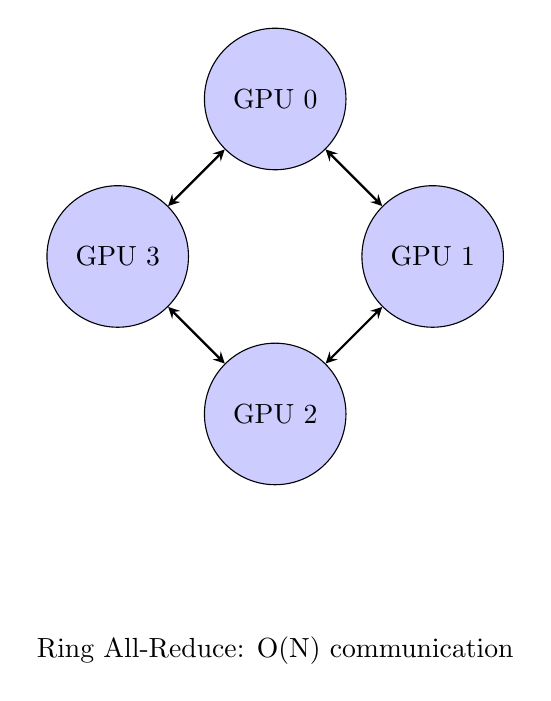
\begin{tikzpicture}[node distance=2.5cm, auto]
    \tikzstyle{worker} = [circle, draw, fill=blue!20, text width=1.5cm, text centered]
    \tikzstyle{arrow} = [thick,<->,>=stealth]

    % Workers in a ring
    \node [worker] (w1) at (0,2) {GPU 0};
    \node [worker] (w2) at (2,0) {GPU 1};
    \node [worker] (w3) at (0,-2) {GPU 2};
    \node [worker] (w4) at (-2,0) {GPU 3};

    % Ring connections
    \draw [arrow] (w1) -- (w2);
    \draw [arrow] (w2) -- (w3);
    \draw [arrow] (w3) -- (w4);
    \draw [arrow] (w4) -- (w1);

    \node [below of=w3, node distance=3cm] {Ring All-Reduce: O(N) communication};
\end{tikzpicture}
\caption{All-reduce architecture (ring topology)}
\label{fig:allreduce}
\end{figure}

\textbf{Advantages:}
\begin{itemize}
    \item No single point of failure
    \item Efficient bandwidth utilization
    \item Simpler implementation
    \item Better for synchronous training
\end{itemize}

\textbf{Disadvantages:}
\begin{itemize}
    \item All workers must participate (synchronous)
    \item Slower workers stall entire system
    \item Fixed topology
\end{itemize}

\section{Gradient Synchronization Strategies}

\subsection{Synchronous SGD}

All workers compute gradients, synchronize, then update together.

\begin{lstlisting}[style=python, caption=Synchronous gradient synchronization]
import torch
import torch.distributed as dist

def synchronous_sgd_step(model, optimizer, loss):
    """Synchronous SGD with gradient averaging"""
    # Backward pass (compute local gradients)
    optimizer.zero_grad()
    loss.backward()

    # Average gradients across all workers
    world_size = dist.get_world_size()
    for param in model.parameters():
        if param.grad is not None:
            # All-reduce sums gradients across workers
            dist.all_reduce(param.grad.data, op=dist.ReduceOp.SUM)
            # Average by dividing by world size
            param.grad.data /= world_size

    # Update parameters (now all workers have same gradients)
    optimizer.step()

# Gradient accumulation for larger effective batch size
def synchronous_sgd_with_accumulation(model, optimizer, loss,
                                     accumulation_steps=4):
    """Synchronous SGD with gradient accumulation"""
    # Scale loss by accumulation steps
    loss = loss / accumulation_steps
    loss.backward()

    # Only synchronize and step every accumulation_steps
    if (step + 1) % accumulation_steps == 0:
        # Synchronize gradients
        world_size = dist.get_world_size()
        for param in model.parameters():
            if param.grad is not None:
                dist.all_reduce(param.grad.data, op=dist.ReduceOp.SUM)
                param.grad.data /= world_size

        # Update
        optimizer.step()
        optimizer.zero_grad()
\end{lstlisting}

\subsection{Asynchronous SGD}

Workers update parameters independently without waiting for others.

\begin{lstlisting}[style=python, caption=Asynchronous parameter server implementation]
import torch
import torch.distributed.rpc as rpc
from torch.distributed.rpc import RRef

class ParameterServer:
    """Centralized parameter server for async SGD"""
    def __init__(self, model):
        self.model = model
        self.optimizer = torch.optim.SGD(model.parameters(), lr=0.01)
        self.lock = threading.Lock()
        self.version = 0

    @staticmethod
    @rpc.functions.async_execution
    def get_parameters(self):
        """Workers fetch current parameters"""
        with self.lock:
            return {
                name: param.data.clone()
                for name, param in self.model.named_parameters()
            }

    @staticmethod
    @rpc.functions.async_execution
    def apply_gradients(self, gradients):
        """Workers push gradients"""
        with self.lock:
            # Apply gradients
            for name, param in self.model.named_parameters():
                if name in gradients:
                    param.grad = gradients[name]

            # Update parameters
            self.optimizer.step()
            self.optimizer.zero_grad()
            self.version += 1

            return self.version

class AsyncWorker:
    """Worker for async SGD"""
    def __init__(self, rank, ps_rref, model, train_loader):
        self.rank = rank
        self.ps_rref = ps_rref
        self.model = model
        self.train_loader = train_loader
        self.criterion = torch.nn.CrossEntropyLoss()

    def train_async(self, num_iterations):
        """Asynchronous training loop"""
        for iteration in range(num_iterations):
            # Fetch latest parameters from PS
            params = self.ps_rref.rpc_sync().get_parameters()

            # Update local model
            for name, param in self.model.named_parameters():
                param.data.copy_(params[name])

            # Compute gradients on local batch
            data, target = next(iter(self.train_loader))
            output = self.model(data)
            loss = self.criterion(output, target)

            self.model.zero_grad()
            loss.backward()

            # Collect gradients
            gradients = {
                name: param.grad.clone()
                for name, param in self.model.named_parameters()
                if param.grad is not None
            }

            # Push gradients to PS (async)
            version = self.ps_rref.rpc_async().apply_gradients(gradients)

            if iteration % 10 == 0:
                print(f'Worker {self.rank} | Iteration {iteration} | '
                      f'Loss: {loss.item():.4f}')
\end{lstlisting}

\subsection{Hogwild! (Lock-Free Async SGD)}

Multiple threads/processes update shared parameters without locks, accepting potential race conditions.

\begin{lstlisting}[style=python, caption=Hogwild implementation]
import torch
import torch.multiprocessing as mp
from torch.multiprocessing import Queue

def hogwild_worker(rank, model, dataset, num_epochs, queue):
    """Lock-free async training worker"""
    # Each worker has reference to shared model parameters
    optimizer = torch.optim.SGD(model.parameters(), lr=0.01)
    criterion = torch.nn.CrossEntropyLoss()

    for epoch in range(num_epochs):
        for batch_idx, (data, target) in enumerate(dataset):
            # Forward pass
            output = model(data)
            loss = criterion(output, target)

            # Backward pass
            optimizer.zero_grad()
            loss.backward()

            # Update (no synchronization - potential race conditions)
            optimizer.step()

            if batch_idx % 10 == 0:
                queue.put((rank, epoch, batch_idx, loss.item()))

def train_hogwild(model, train_loader, num_workers=4, num_epochs=10):
    """Hogwild training with multiple workers"""
    # Share model parameters across processes
    model.share_memory()

    # Create queue for logging
    queue = Queue()

    # Spawn workers
    processes = []
    for rank in range(num_workers):
        p = mp.Process(
            target=hogwild_worker,
            args=(rank, model, train_loader, num_epochs, queue)
        )
        p.start()
        processes.append(p)

    # Monitor progress
    while any(p.is_alive() for p in processes):
        if not queue.empty():
            rank, epoch, batch, loss = queue.get()
            print(f'Worker {rank} | Epoch {epoch} | Batch {batch} | Loss: {loss:.4f}')

    # Wait for completion
    for p in processes:
        p.join()
\end{lstlisting}

\section{Horovod: Framework-Agnostic Distributed Training}

Horovod provides a unified API for distributed training across TensorFlow, PyTorch, and MXNet.

\begin{lstlisting}[style=python, caption=Horovod distributed training]
import torch
import horovod.torch as hvd

# Initialize Horovod
hvd.init()

# Pin GPU to local rank
torch.cuda.set_device(hvd.local_rank())

# Build model
model = ResNet50().cuda()

# Scale learning rate by number of workers
optimizer = torch.optim.SGD(
    model.parameters(),
    lr=0.01 * hvd.size(),  # Scale LR
    momentum=0.9
)

# Wrap optimizer with Horovod DistributedOptimizer
optimizer = hvd.DistributedOptimizer(
    optimizer,
    named_parameters=model.named_parameters(),
    backward_passes_per_step=1
)

# Broadcast parameters from rank 0
hvd.broadcast_parameters(model.state_dict(), root_rank=0)
hvd.broadcast_optimizer_state(optimizer, root_rank=0)

# Create distributed sampler
train_sampler = torch.utils.data.distributed.DistributedSampler(
    train_dataset,
    num_replicas=hvd.size(),
    rank=hvd.rank()
)

train_loader = torch.utils.data.DataLoader(
    train_dataset,
    batch_size=64,
    sampler=train_sampler
)

# Training loop
for epoch in range(100):
    train_sampler.set_epoch(epoch)

    for batch_idx, (data, target) in enumerate(train_loader):
        data, target = data.cuda(), target.cuda()

        optimizer.zero_grad()
        output = model(data)
        loss = criterion(output, target)
        loss.backward()

        # Horovod handles gradient averaging
        optimizer.step()

        if hvd.rank() == 0 and batch_idx % 10 == 0:
            print(f'Epoch {epoch} | Batch {batch_idx} | Loss: {loss.item():.4f}')

# Launch with horovodrun
# horovodrun -np 4 python train_horovod.py
# horovodrun -np 8 -H server1:4,server2:4 python train_horovod.py
\end{lstlisting}

\subsection{Horovod Timeline for Performance Analysis}

\begin{lstlisting}[style=python, caption=Horovod performance profiling]
import horovod.torch as hvd

# Enable timeline
hvd.init()

# Set environment variable before running
# export HOROVOD_TIMELINE=timeline.json

# Training code here...

# Analyze timeline
# chrome://tracing in Chrome browser
# Load timeline.json to visualize:
# - Communication vs computation time
# - Gradient synchronization patterns
# - Bottlenecks and stragglers
\end{lstlisting}

\section{Ray for Flexible Distributed Training}

Ray provides flexible distributed computing primitives for ML workloads.

\begin{lstlisting}[style=python, caption=Distributed training with Ray]
import ray
from ray import train
from ray.train import ScalingConfig
from ray.train.torch import TorchTrainer
import torch
import torch.nn as nn

def train_func(config):
    """Training function that runs on each worker"""
    # Get distributed context
    rank = train.get_context().get_world_rank()
    world_size = train.get_context().get_world_size()

    # Build model
    model = ResNet50()
    model = train.torch.prepare_model(model)  # Wraps with DDP

    # Optimizer
    optimizer = torch.optim.SGD(
        model.parameters(),
        lr=config['lr'],
        momentum=0.9
    )

    # Data loader
    train_dataset = get_dataset()
    train_loader = torch.utils.data.DataLoader(
        train_dataset,
        batch_size=config['batch_size'],
        shuffle=True
    )
    train_loader = train.torch.prepare_data_loader(train_loader)

    # Training loop
    for epoch in range(config['num_epochs']):
        model.train()
        total_loss = 0

        for batch_idx, (data, target) in enumerate(train_loader):
            optimizer.zero_grad()
            output = model(data)
            loss = nn.CrossEntropyLoss()(output, target)
            loss.backward()
            optimizer.step()

            total_loss += loss.item()

        avg_loss = total_loss / len(train_loader)

        # Report metrics to Ray
        train.report({"loss": avg_loss, "epoch": epoch})

# Create Ray trainer
trainer = TorchTrainer(
    train_loop_per_worker=train_func,
    train_loop_config={
        "lr": 0.01,
        "batch_size": 64,
        "num_epochs": 100
    },
    scaling_config=ScalingConfig(
        num_workers=4,
        use_gpu=True,
        resources_per_worker={"CPU": 4, "GPU": 1}
    )
)

# Run training
result = trainer.fit()
print(f"Final metrics: {result.metrics}")

# Advanced: Hyperparameter tuning with Ray Tune
from ray import tune

param_space = {
    "train_loop_config": {
        "lr": tune.loguniform(1e-4, 1e-1),
        "batch_size": tune.choice([32, 64, 128]),
        "num_epochs": 100
    }
}

tuner = tune.Tuner(
    trainer,
    param_space=param_space,
    tune_config=tune.TuneConfig(
        metric="loss",
        mode="min",
        num_samples=10
    )
)

results = tuner.fit()
best_result = results.get_best_result()
print(f"Best hyperparameters: {best_result.config}")
\end{lstlisting}

\section{Fault Tolerance and Checkpointing}

Production distributed training must handle failures gracefully.

\begin{lstlisting}[style=python, caption=Fault-tolerant training with elastic checkpointing]
import torch
import torch.distributed as dist
import os
from datetime import datetime
import time

class ElasticCheckpointer:
    """Fault-tolerant checkpointing for distributed training"""

    def __init__(self, checkpoint_dir, save_frequency=10):
        self.checkpoint_dir = checkpoint_dir
        self.save_frequency = save_frequency
        os.makedirs(checkpoint_dir, exist_ok=True)

    def save_checkpoint(self, epoch, model, optimizer, scheduler,
                       metrics, rank):
        """Save checkpoint with atomic write"""
        if rank != 0:
            return  # Only rank 0 saves

        checkpoint = {
            'epoch': epoch,
            'model_state_dict': model.module.state_dict(),
            'optimizer_state_dict': optimizer.state_dict(),
            'scheduler_state_dict': scheduler.state_dict(),
            'metrics': metrics,
            'timestamp': datetime.now().isoformat()
        }

        # Atomic save: write to temp file, then rename
        temp_path = os.path.join(
            self.checkpoint_dir,
            f'checkpoint_temp_{epoch}.pth'
        )
        final_path = os.path.join(
            self.checkpoint_dir,
            f'checkpoint_epoch_{epoch}.pth'
        )

        # Save to temp file
        torch.save(checkpoint, temp_path)

        # Atomic rename
        os.replace(temp_path, final_path)

        # Update latest symlink
        latest_path = os.path.join(self.checkpoint_dir, 'checkpoint_latest.pth')
        if os.path.exists(latest_path):
            os.remove(latest_path)
        os.symlink(final_path, latest_path)

        print(f'Checkpoint saved: {final_path}')

        # Clean old checkpoints (keep last 5)
        self.cleanup_old_checkpoints(keep=5)

    def load_checkpoint(self, model, optimizer=None, scheduler=None):
        """Load latest checkpoint"""
        latest_path = os.path.join(self.checkpoint_dir, 'checkpoint_latest.pth')

        if not os.path.exists(latest_path):
            print('No checkpoint found, starting from scratch')
            return 0, {}

        print(f'Loading checkpoint: {latest_path}')
        checkpoint = torch.load(latest_path)

        # Load model state
        model.module.load_state_dict(checkpoint['model_state_dict'])

        # Load optimizer state
        if optimizer and 'optimizer_state_dict' in checkpoint:
            optimizer.load_state_dict(checkpoint['optimizer_state_dict'])

        # Load scheduler state
        if scheduler and 'scheduler_state_dict' in checkpoint:
            scheduler.load_state_dict(checkpoint['scheduler_state_dict'])

        print(f"Resumed from epoch {checkpoint['epoch']}")

        return checkpoint['epoch'], checkpoint.get('metrics', {})

    def cleanup_old_checkpoints(self, keep=5):
        """Remove old checkpoints, keeping only the latest N"""
        checkpoints = sorted([
            f for f in os.listdir(self.checkpoint_dir)
            if f.startswith('checkpoint_epoch_') and f.endswith('.pth')
        ])

        if len(checkpoints) > keep:
            for old_checkpoint in checkpoints[:-keep]:
                path = os.path.join(self.checkpoint_dir, old_checkpoint)
                os.remove(path)
                print(f'Removed old checkpoint: {path}')

def train_with_fault_tolerance(rank, world_size):
    """Training with automatic restart on failure"""
    # Setup
    setup_distributed(rank, world_size)

    model = ResNet50().cuda(rank)
    model = DDP(model, device_ids=[rank])

    optimizer = torch.optim.SGD(model.parameters(), lr=0.1)
    scheduler = torch.optim.lr_scheduler.StepLR(optimizer, step_size=30)

    # Checkpointer
    checkpointer = ElasticCheckpointer(
        checkpoint_dir='./checkpoints',
        save_frequency=10
    )

    # Resume from checkpoint
    start_epoch, _ = checkpointer.load_checkpoint(
        model, optimizer, scheduler
    )

    # Training loop with fault handling
    for epoch in range(start_epoch, 100):
        try:
            # Training code
            train_loss = train_epoch(model, train_loader, optimizer, rank)
            val_loss = validate(model, val_loader, rank)
            scheduler.step()

            # Save checkpoint
            if (epoch + 1) % checkpointer.save_frequency == 0:
                metrics = {
                    'train_loss': train_loss,
                    'val_loss': val_loss,
                    'lr': scheduler.get_last_lr()[0]
                }
                checkpointer.save_checkpoint(
                    epoch, model, optimizer, scheduler, metrics, rank
                )

        except RuntimeError as e:
            if "out of memory" in str(e):
                print(f"OOM error at epoch {epoch}, saving checkpoint...")
                # Save emergency checkpoint
                checkpointer.save_checkpoint(
                    epoch, model, optimizer, scheduler, {}, rank
                )
                # Clear cache and retry
                torch.cuda.empty_cache()
                continue
            else:
                raise

        except Exception as e:
            # Save checkpoint on unexpected error
            print(f"Error at epoch {epoch}: {e}")
            checkpointer.save_checkpoint(
                epoch, model, optimizer, scheduler, {}, rank
            )
            raise

    cleanup_distributed()

# Elastic training with automatic restart
def elastic_train_with_auto_restart():
    """Wrapper that restarts training on failure"""
    max_retries = 3
    retry_count = 0

    while retry_count < max_retries:
        try:
            world_size = torch.cuda.device_count()
            mp.spawn(
                train_with_fault_tolerance,
                args=(world_size,),
                nprocs=world_size,
                join=True
            )
            print("Training completed successfully")
            break

        except Exception as e:
            retry_count += 1
            print(f"Training failed (attempt {retry_count}/{max_retries}): {e}")

            if retry_count < max_retries:
                print(f"Restarting in 10 seconds...")
                time.sleep(10)
            else:
                print("Max retries reached, giving up")
                raise
\end{lstlisting}

\section{Performance Benchmarking and Optimization}

\subsection{Measuring Distributed Training Performance}

\begin{lstlisting}[style=python, caption=Comprehensive performance benchmarking]
import torch
import time
from contextlib import contextmanager
import numpy as np

class DistributedTrainingBenchmark:
    """Benchmark distributed training performance"""

    def __init__(self, rank, world_size):
        self.rank = rank
        self.world_size = world_size
        self.metrics = {}

    @contextmanager
    def timer(self, name):
        """Context manager for timing code blocks"""
        start = time.perf_counter()
        yield
        elapsed = time.perf_counter() - start

        if name not in self.metrics:
            self.metrics[name] = []
        self.metrics[name].append(elapsed)

    def benchmark_epoch(self, model, dataloader, criterion, optimizer):
        """Benchmark one training epoch with detailed metrics"""
        model.train()

        epoch_metrics = {
            'forward_time': [],
            'backward_time': [],
            'optimizer_time': [],
            'data_loading_time': [],
            'communication_time': []
        }

        batch_start = time.perf_counter()

        for batch_idx, (data, target) in enumerate(dataloader):
            # Data loading time
            data_time = time.perf_counter() - batch_start
            epoch_metrics['data_loading_time'].append(data_time)

            data = data.cuda(self.rank, non_blocking=True)
            target = target.cuda(self.rank, non_blocking=True)

            # Forward pass
            forward_start = time.perf_counter()
            optimizer.zero_grad(set_to_none=True)
            output = model(data)
            loss = criterion(output, target)
            forward_time = time.perf_counter() - forward_start
            epoch_metrics['forward_time'].append(forward_time)

            # Backward pass
            backward_start = time.perf_counter()
            loss.backward()
            backward_time = time.perf_counter() - backward_start
            epoch_metrics['backward_time'].append(backward_time)

            # Communication time (gradient synchronization in DDP)
            comm_start = time.perf_counter()
            # DDP automatically syncs gradients during backward
            # This measures the explicit sync if needed
            torch.cuda.synchronize()
            comm_time = time.perf_counter() - comm_start
            epoch_metrics['communication_time'].append(comm_time)

            # Optimizer step
            opt_start = time.perf_counter()
            optimizer.step()
            torch.cuda.synchronize()
            opt_time = time.perf_counter() - opt_start
            epoch_metrics['optimizer_time'].append(opt_time)

            batch_start = time.perf_counter()

        return epoch_metrics

    def compute_statistics(self, metrics):
        """Compute statistics across all batches"""
        stats = {}
        for metric_name, values in metrics.items():
            values = np.array(values)
            stats[metric_name] = {
                'mean': values.mean(),
                'std': values.std(),
                'min': values.min(),
                'max': values.max(),
                'p50': np.percentile(values, 50),
                'p95': np.percentile(values, 95),
                'p99': np.percentile(values, 99)
            }
        return stats

    def print_report(self, stats):
        """Print performance report"""
        if self.rank == 0:
            print("\n" + "="*70)
            print("Distributed Training Performance Report")
            print("="*70)
            print(f"World Size: {self.world_size} GPUs")
            print()

            for metric_name, metric_stats in stats.items():
                print(f"{metric_name}:")
                print(f"  Mean: {metric_stats['mean']*1000:.2f} ms")
                print(f"  Std:  {metric_stats['std']*1000:.2f} ms")
                print(f"  P50:  {metric_stats['p50']*1000:.2f} ms")
                print(f"  P95:  {metric_stats['p95']*1000:.2f} ms")
                print(f"  P99:  {metric_stats['p99']*1000:.2f} ms")
                print()

            # Compute efficiency metrics
            total_time_per_batch = sum(
                s['mean'] for s in stats.values()
            )
            compute_time = (
                stats['forward_time']['mean'] +
                stats['backward_time']['mean'] +
                stats['optimizer_time']['mean']
            )
            comm_time = stats['communication_time']['mean']

            compute_ratio = compute_time / total_time_per_batch * 100
            comm_ratio = comm_time / total_time_per_batch * 100

            print(f"Efficiency Analysis:")
            print(f"  Computation: {compute_ratio:.1f}%")
            print(f"  Communication: {comm_ratio:.1f}%")
            print(f"  Data Loading: {stats['data_loading_time']['mean']/total_time_per_batch*100:.1f}%")
            print()

            # Throughput
            samples_per_sec = 1.0 / total_time_per_batch * self.world_size
            print(f"Throughput:")
            print(f"  Samples/sec (per GPU): {samples_per_sec:.2f}")
            print(f"  Samples/sec (total): {samples_per_sec * self.world_size:.2f}")
            print("="*70 + "\n")

    def measure_communication_overhead(self, tensor_size=(1024, 1024)):
        """Measure pure communication overhead"""
        tensor = torch.randn(tensor_size).cuda(self.rank)

        # Warmup
        for _ in range(10):
            dist.all_reduce(tensor)

        torch.cuda.synchronize()

        # Measure
        times = []
        for _ in range(100):
            start = time.perf_counter()
            dist.all_reduce(tensor)
            torch.cuda.synchronize()
            elapsed = time.perf_counter() - start
            times.append(elapsed)

        if self.rank == 0:
            print(f"\nAll-Reduce Communication Benchmark:")
            print(f"  Tensor size: {tensor_size}")
            print(f"  Mean latency: {np.mean(times)*1000:.2f} ms")
            print(f"  Bandwidth: {tensor.element_size() * tensor.numel() / np.mean(times) / 1e9:.2f} GB/s")

def scaling_efficiency_benchmark():
    """Benchmark scaling efficiency across different GPU counts"""
    model = ResNet50()

    results = {}

    for num_gpus in [1, 2, 4, 8]:
        # Run training with num_gpus
        # Measure throughput
        throughput = measure_throughput(model, num_gpus)
        results[num_gpus] = throughput

    # Compute scaling efficiency
    baseline = results[1]

    print("\nScaling Efficiency:")
    print(f"{'GPUs':<10} {'Throughput':<15} {'Speedup':<15} {'Efficiency':<15}")
    print("-" * 60)

    for num_gpus, throughput in results.items():
        speedup = throughput / baseline
        efficiency = speedup / num_gpus
        print(f"{num_gpus:<10} {throughput:<15.2f} {speedup:<15.2f} {efficiency*100:<15.1f}%")
\end{lstlisting}

\subsection{Identifying and Resolving Bottlenecks}

\begin{lstlisting}[style=python, caption=Bottleneck detection and optimization]
import torch
from torch.profiler import profile, ProfilerActivity, schedule

def profile_distributed_training(model, dataloader, num_steps=100):
    """Profile distributed training to identify bottlenecks"""

    # Create profiler with schedule
    prof_schedule = schedule(
        wait=5,      # Skip first 5 steps
        warmup=5,    # Warmup for 5 steps
        active=10,   # Profile 10 steps
        repeat=2     # Repeat cycle 2 times
    )

    with profile(
        activities=[ProfilerActivity.CPU, ProfilerActivity.CUDA],
        schedule=prof_schedule,
        on_trace_ready=torch.profiler.tensorboard_trace_handler('./profiler_logs'),
        record_shapes=True,
        profile_memory=True,
        with_stack=True
    ) as prof:

        for step, (data, target) in enumerate(dataloader):
            if step >= num_steps:
                break

            data = data.cuda(non_blocking=True)
            target = target.cuda(non_blocking=True)

            output = model(data)
            loss = nn.CrossEntropyLoss()(output, target)
            loss.backward()
            optimizer.step()
            optimizer.zero_grad()

            prof.step()

    # Print summary
    print(prof.key_averages().table(
        sort_by="cuda_time_total",
        row_limit=20
    ))

    # Export for visualization
    # tensorboard --logdir=./profiler_logs

# Optimization tips based on profiling results:

def optimize_data_loading():
    """Optimize data loading bottleneck"""
    dataloader = DataLoader(
        dataset,
        batch_size=64,
        num_workers=4,           # Parallel data loading
        pin_memory=True,         # Faster GPU transfer
        persistent_workers=True, # Keep workers alive
        prefetch_factor=2        # Prefetch batches
    )
    return dataloader

def optimize_gradient_communication():
    """Optimize gradient synchronization"""
    # Use gradient compression (requires apex)
    # from apex import amp
    # model, optimizer = amp.initialize(model, optimizer, opt_level="O1")

    # Or use gradient bucketing (built into DDP)
    model = DDP(
        model,
        device_ids=[rank],
        bucket_cap_mb=25,  # Larger buckets = fewer all-reduces
        gradient_as_bucket_view=True
    )

    return model

def optimize_mixed_precision():
    """Use automatic mixed precision"""
    from torch.cuda.amp import autocast, GradScaler

    scaler = GradScaler()

    for data, target in dataloader:
        optimizer.zero_grad()

        # Forward in mixed precision
        with autocast():
            output = model(data)
            loss = criterion(output, target)

        # Backward with gradient scaling
        scaler.scale(loss).backward()
        scaler.step(optimizer)
        scaler.update()
\end{lstlisting}

\section{Resource Allocation and Scheduling}

\subsection{SLURM Job Scheduling}

\begin{lstlisting}[style=shell, caption=SLURM batch script for distributed training]
#!/bin/bash
#SBATCH --job-name=distributed_training
#SBATCH --nodes=4
#SBATCH --ntasks-per-node=4
#SBATCH --cpus-per-task=8
#SBATCH --gres=gpu:4
#SBATCH --time=48:00:00
#SBATCH --partition=gpu
#SBATCH --output=logs/train_%j.out
#SBATCH --error=logs/train_%j.err

# Load modules
module load cuda/11.8
module load python/3.9

# Activate environment
source ~/venv/bin/activate

# Get master node
export MASTER_ADDR=$(scontrol show hostname ${SLURM_NODELIST} | head -n 1)
export MASTER_PORT=12355

# Launch training
srun python -u train_distributed.py \
    --epochs 100 \
    --batch-size 64 \
    --lr 0.1 \
    --checkpoint-dir checkpoints/

# Post-processing
python evaluate_model.py --checkpoint checkpoints/checkpoint_best.pth
\end{lstlisting}

\subsection{Kubernetes Job Specification}

\begin{lstlisting}[style=yaml, caption=Kubernetes PyTorchJob for distributed training]
apiVersion: kubeflow.org/v1
kind: PyTorchJob
metadata:
  name: distributed-training
  namespace: ml-workloads
spec:
  pytorchReplicaSpecs:
    Master:
      replicas: 1
      restartPolicy: OnFailure
      template:
        spec:
          containers:
          - name: pytorch
            image: pytorch/pytorch:2.0.0-cuda11.8-cudnn8-runtime
            command:
              - python
              - -u
              - train_distributed.py
            args:
              - --epochs=100
              - --batch-size=64
            resources:
              limits:
                nvidia.com/gpu: 1
                memory: 32Gi
                cpu: 8
              requests:
                nvidia.com/gpu: 1
                memory: 16Gi
                cpu: 4
            volumeMounts:
            - name: data
              mountPath: /data
            - name: checkpoints
              mountPath: /checkpoints
          volumes:
          - name: data
            persistentVolumeClaim:
              claimName: training-data-pvc
          - name: checkpoints
            persistentVolumeClaim:
              claimName: checkpoint-pvc

    Worker:
      replicas: 3
      restartPolicy: OnFailure
      template:
        spec:
          containers:
          - name: pytorch
            image: pytorch/pytorch:2.0.0-cuda11.8-cudnn8-runtime
            command:
              - python
              - -u
              - train_distributed.py
            args:
              - --epochs=100
              - --batch-size=64
            resources:
              limits:
                nvidia.com/gpu: 1
                memory: 32Gi
                cpu: 8
              requests:
                nvidia.com/gpu: 1
                memory: 16Gi
                cpu: 4
            volumeMounts:
            - name: data
              mountPath: /data
            - name: checkpoints
              mountPath: /checkpoints
          volumes:
          - name: data
            persistentVolumeClaim:
              claimName: training-data-pvc
          - name: checkpoints
            persistentVolumeClaim:
              claimName: checkpoint-pvc
\end{lstlisting}

\section{Memory Management in Distributed Settings}

Efficient memory management is critical for distributed training, especially for large models. This section covers techniques for optimizing memory usage across GPUs.

\subsection{Gradient Checkpointing}

Gradient checkpointing trades computation for memory by recomputing activations during backward pass instead of storing them.

\begin{lstlisting}[style=python, caption=Gradient checkpointing implementation]
import torch
import torch.nn as nn
from torch.utils.checkpoint import checkpoint

class CheckpointedResidualBlock(nn.Module):
    """Residual block with gradient checkpointing"""
    def __init__(self, channels):
        super().__init__()
        self.conv1 = nn.Conv2d(channels, channels, 3, padding=1)
        self.bn1 = nn.BatchNorm2d(channels)
        self.conv2 = nn.Conv2d(channels, channels, 3, padding=1)
        self.bn2 = nn.BatchNorm2d(channels)
        self.relu = nn.ReLU(inplace=True)

    def forward(self, x):
        # Checkpoint this block to save memory
        return checkpoint(self._forward, x, use_reentrant=False)

    def _forward(self, x):
        identity = x
        out = self.conv1(x)
        out = self.bn1(out)
        out = self.relu(out)
        out = self.conv2(out)
        out = self.bn2(out)
        out += identity
        out = self.relu(out)
        return out

# Transformer with selective checkpointing
class CheckpointedTransformerLayer(nn.Module):
    """Transformer layer with gradient checkpointing"""
    def __init__(self, d_model, nhead, dim_feedforward):
        super().__init__()
        self.self_attn = nn.MultiheadAttention(d_model, nhead)
        self.linear1 = nn.Linear(d_model, dim_feedforward)
        self.linear2 = nn.Linear(dim_feedforward, d_model)
        self.norm1 = nn.LayerNorm(d_model)
        self.norm2 = nn.LayerNorm(d_model)
        self.dropout = nn.Dropout(0.1)

    def forward(self, src):
        # Checkpoint attention and feedforward
        src2 = checkpoint(self._attention_block, src, use_reentrant=False)
        src = src + self.dropout(src2)
        src = self.norm1(src)

        src2 = checkpoint(self._feedforward_block, src, use_reentrant=False)
        src = src + self.dropout(src2)
        src = self.norm2(src)

        return src

    def _attention_block(self, src):
        return self.self_attn(src, src, src)[0]

    def _feedforward_block(self, src):
        src2 = self.linear2(torch.relu(self.linear1(src)))
        return src2

# Memory usage comparison
def measure_memory_usage():
    """Compare memory usage with and without checkpointing"""
    import torch.cuda as cuda

    # Without checkpointing
    model_no_cp = nn.Sequential(*[
        ResidualBlock(256) for _ in range(50)
    ]).cuda()

    cuda.reset_peak_memory_stats()
    x = torch.randn(32, 256, 56, 56).cuda()
    y = model_no_cp(x)
    y.sum().backward()
    memory_no_cp = cuda.max_memory_allocated() / 1e9  # GB

    # With checkpointing
    model_cp = nn.Sequential(*[
        CheckpointedResidualBlock(256) for _ in range(50)
    ]).cuda()

    cuda.reset_peak_memory_stats()
    x = torch.randn(32, 256, 56, 56).cuda()
    y = model_cp(x)
    y.sum().backward()
    memory_cp = cuda.max_memory_allocated() / 1e9  # GB

    print(f"Memory without checkpointing: {memory_no_cp:.2f} GB")
    print(f"Memory with checkpointing: {memory_cp:.2f} GB")
    print(f"Memory saved: {(1 - memory_cp/memory_no_cp)*100:.1f}%")
\end{lstlisting}

\subsection{ZeRO: Zero Redundancy Optimizer}

ZeRO (from Microsoft DeepSpeed) partitions optimizer states, gradients, and parameters across devices to reduce memory redundancy.

\begin{lstlisting}[style=python, caption=DeepSpeed ZeRO optimization]
import torch
import deepspeed
from deepspeed.ops.adam import DeepSpeedCPUAdam

# DeepSpeed configuration
ds_config = {
    "train_batch_size": 64,
    "train_micro_batch_size_per_gpu": 8,
    "gradient_accumulation_steps": 8,

    # ZeRO optimization
    "zero_optimization": {
        "stage": 3,  # Stage 0, 1, 2, or 3
        # Stage 1: Partition optimizer states
        # Stage 2: Partition optimizer states + gradients
        # Stage 3: Partition optimizer states + gradients + parameters

        "offload_optimizer": {
            "device": "cpu",  # Offload to CPU
            "pin_memory": True
        },
        "offload_param": {
            "device": "cpu",
            "pin_memory": True
        },

        "overlap_comm": True,  # Overlap communication with computation
        "contiguous_gradients": True,
        "reduce_bucket_size": 5e7,
        "stage3_prefetch_bucket_size": 5e7,
        "stage3_param_persistence_threshold": 1e5,
    },

    # Mixed precision training
    "fp16": {
        "enabled": True,
        "loss_scale": 0,
        "initial_scale_power": 16,
        "loss_scale_window": 1000,
        "hysteresis": 2,
        "min_loss_scale": 1
    },

    # Gradient clipping
    "gradient_clipping": 1.0,

    # Logging
    "steps_per_print": 100,
    "wall_clock_breakdown": False
}

# Initialize model
model = TransformerModel(
    vocab_size=50000,
    d_model=1024,
    nhead=16,
    num_layers=24
)

# Initialize DeepSpeed
model_engine, optimizer, train_loader, _ = deepspeed.initialize(
    model=model,
    model_parameters=model.parameters(),
    config=ds_config,
    training_data=train_dataset
)

# Training loop
for epoch in range(num_epochs):
    for batch in train_loader:
        inputs, labels = batch

        # Forward pass
        outputs = model_engine(inputs)
        loss = criterion(outputs, labels)

        # Backward pass (DeepSpeed handles ZeRO partitioning)
        model_engine.backward(loss)

        # Optimizer step
        model_engine.step()

# Save checkpoint
model_engine.save_checkpoint('checkpoints/')

# Memory comparison:
# - Without ZeRO Stage 3: ~32 GB per GPU for 1B parameter model
# - With ZeRO Stage 3: ~8 GB per GPU for same model
# - Can train 4x larger models on same hardware
\end{lstlisting}

\subsection{Activation Memory Optimization}

\begin{lstlisting}[style=python, caption=Techniques for reducing activation memory]
import torch
import torch.nn as nn

class MemoryEfficientAttention(nn.Module):
    """
    Memory-efficient attention using Flash Attention.
    Reduces memory from O(N^2) to O(N) for sequence length N.
    """
    def __init__(self, d_model, nhead):
        super().__init__()
        self.d_model = d_model
        self.nhead = nhead
        self.head_dim = d_model // nhead

        self.q_proj = nn.Linear(d_model, d_model)
        self.k_proj = nn.Linear(d_model, d_model)
        self.v_proj = nn.Linear(d_model, d_model)
        self.out_proj = nn.Linear(d_model, d_model)

    def forward(self, x):
        batch_size, seq_len, _ = x.shape

        # Project Q, K, V
        q = self.q_proj(x).view(batch_size, seq_len, self.nhead, self.head_dim)
        k = self.k_proj(x).view(batch_size, seq_len, self.nhead, self.head_dim)
        v = self.v_proj(x).view(batch_size, seq_len, self.nhead, self.head_dim)

        # Use Flash Attention (if available)
        try:
            from flash_attn import flash_attn_func
            # Flash attention computes in blocks, reducing memory
            out = flash_attn_func(q, k, v, dropout_p=0.0, causal=False)
        except ImportError:
            # Fallback to memory-efficient attention
            out = self._efficient_attention(q, k, v)

        out = out.reshape(batch_size, seq_len, self.d_model)
        return self.out_proj(out)

    def _efficient_attention(self, q, k, v):
        """Memory-efficient attention using chunking"""
        batch_size, seq_len, nhead, head_dim = q.shape
        chunk_size = 512  # Process in chunks

        outputs = []
        for i in range(0, seq_len, chunk_size):
            q_chunk = q[:, i:i+chunk_size]

            # Compute attention for this chunk
            scores = torch.matmul(
                q_chunk.transpose(1, 2),  # (batch, nhead, chunk, head_dim)
                k.transpose(1, 2).transpose(-2, -1)  # (batch, nhead, head_dim, seq_len)
            ) / (head_dim ** 0.5)

            attn = torch.softmax(scores, dim=-1)
            out = torch.matmul(attn, v.transpose(1, 2))  # (batch, nhead, chunk, head_dim)
            outputs.append(out)

        return torch.cat(outputs, dim=2).transpose(1, 2)

# Inplace operations to save memory
class InplaceOptimizedModel(nn.Module):
    """Use inplace operations where possible"""
    def __init__(self):
        super().__init__()
        self.conv1 = nn.Conv2d(3, 64, 3, padding=1)
        self.bn1 = nn.BatchNorm2d(64)
        self.relu = nn.ReLU(inplace=True)  # Inplace ReLU
        self.conv2 = nn.Conv2d(64, 128, 3, padding=1)
        self.bn2 = nn.BatchNorm2d(128)

    def forward(self, x):
        x = self.conv1(x)
        x = self.bn1(x)
        x = self.relu(x)  # Modifies x in-place
        x = self.conv2(x)
        x = self.bn2(x)
        x = self.relu(x)
        return x

# Mixed precision training for memory savings
from torch.cuda.amp import autocast, GradScaler

def train_with_mixed_precision(model, train_loader):
    """
    Mixed precision training:
    - FP16 for forward/backward (2x less memory)
    - FP32 for optimizer states and critical operations
    """
    scaler = GradScaler()
    optimizer = torch.optim.Adam(model.parameters())

    for data, target in train_loader:
        optimizer.zero_grad()

        # Forward in FP16
        with autocast():
            output = model(data)
            loss = criterion(output, target)

        # Backward with scaled gradients
        scaler.scale(loss).backward()

        # Unscale before clipping
        scaler.unscale_(optimizer)
        torch.nn.utils.clip_grad_norm_(model.parameters(), max_norm=1.0)

        # Step with scaled gradients
        scaler.step(optimizer)
        scaler.update()
\end{lstlisting}

\section{Communication Optimization}

Communication overhead is often the bottleneck in distributed training. This section covers advanced optimization techniques.

\subsection{Gradient Compression}

\begin{lstlisting}[style=python, caption=Gradient compression techniques]
import torch
import torch.distributed as dist

class GradientCompressor:
    """Compress gradients before communication"""

    @staticmethod
    def topk_compression(tensor, compression_ratio=0.01):
        """
        Top-K sparsification: Only communicate largest K% of gradients.
        Reduces communication by 100x with minimal accuracy loss.
        """
        numel = tensor.numel()
        k = max(1, int(numel * compression_ratio))

        # Find top-k absolute values
        _, indices = torch.topk(tensor.abs().flatten(), k)
        values = tensor.flatten()[indices]

        # Create sparse tensor
        compressed = torch.zeros_like(tensor.flatten())
        compressed[indices] = values

        return compressed.view_as(tensor), indices

    @staticmethod
    def quantization_compression(tensor, num_bits=8):
        """
        Quantize gradients to reduce precision.
        8-bit: 4x compression, 4-bit: 8x compression
        """
        # Find min/max
        min_val = tensor.min()
        max_val = tensor.max()

        # Quantize to num_bits
        num_levels = 2 ** num_bits - 1
        scale = (max_val - min_val) / num_levels

        quantized = ((tensor - min_val) / scale).round().to(torch.int16)

        # Dequantize
        dequantized = quantized.to(tensor.dtype) * scale + min_val

        return dequantized, (min_val, max_val, scale)

    @staticmethod
    def powerSGD_compression(tensor, rank=4):
        """
        PowerSGD: Low-rank approximation of gradient matrix.
        Particularly effective for large weight matrices.
        """
        if tensor.dim() < 2:
            return tensor

        # Reshape to 2D if needed
        original_shape = tensor.shape
        if tensor.dim() > 2:
            tensor = tensor.flatten(1)

        m, n = tensor.shape

        # Low-rank approximation: G ≈ P @ Q^T
        # where P is m x rank and Q is n x rank
        U, S, Vh = torch.linalg.svd(tensor, full_matrices=False)

        # Keep only top 'rank' components
        P = U[:, :rank] @ torch.diag(S[:rank].sqrt())
        Q = (Vh[:rank, :].T @ torch.diag(S[:rank].sqrt()))

        # Reconstruct
        compressed = P @ Q.T

        return compressed.reshape(original_shape)

# Use compression in distributed training
class CompressedDDP(nn.Module):
    """DDP with gradient compression"""
    def __init__(self, model, compression_ratio=0.01):
        super().__init__()
        self.model = model
        self.compression_ratio = compression_ratio
        self.compressor = GradientCompressor()

    def forward(self, *args, **kwargs):
        return self.model(*args, **kwargs)

    def backward_with_compression(self, loss):
        """Backward with compressed gradient communication"""
        loss.backward()

        # Compress and communicate gradients
        for param in self.model.parameters():
            if param.grad is not None:
                # Compress
                compressed_grad, _ = self.compressor.topk_compression(
                    param.grad,
                    self.compression_ratio
                )

                # Communicate compressed gradients
                dist.all_reduce(compressed_grad)

                # Average
                compressed_grad /= dist.get_world_size()

                # Update grad
                param.grad.copy_(compressed_grad)

# Hierarchical All-Reduce for multi-node training
def hierarchical_all_reduce(tensor, local_group, global_group):
    """
    Two-level all-reduce:
    1. All-reduce within node (fast NVLink)
    2. All-reduce across nodes (slower network)

    Reduces inter-node communication.
    """
    # Local all-reduce (within node, fast)
    dist.all_reduce(tensor, group=local_group)
    tensor /= dist.get_world_size(local_group)

    # Select one GPU per node for global communication
    if dist.get_rank(local_group) == 0:
        # Global all-reduce (across nodes)
        dist.all_reduce(tensor, group=global_group)
        tensor /= dist.get_world_size(global_group)

    # Broadcast result within node
    dist.broadcast(tensor, src=0, group=local_group)
\end{lstlisting}

\subsection{Overlapping Computation and Communication}

\begin{lstlisting}[style=python, caption=Overlap communication with computation]
import torch
import torch.distributed as dist
from typing import List

class OverlappedGradientCommunication:
    """
    Overlap gradient communication with backward pass.
    Start communicating gradients for earlier layers while
    still computing gradients for later layers.
    """

    def __init__(self, model, bucket_size_mb=25):
        self.model = model
        self.bucket_size_mb = bucket_size_mb
        self.gradient_buckets: List[List[torch.Tensor]] = []
        self.communication_handles = []

        self._register_hooks()

    def _register_hooks(self):
        """Register backward hooks to trigger async communication"""
        def hook_fn(grad):
            # Trigger async all-reduce when gradient is ready
            handle = dist.all_reduce(grad, async_op=True)
            self.communication_handles.append(handle)
            return grad

        for param in self.model.parameters():
            if param.requires_grad:
                param.register_hook(hook_fn)

    def synchronize(self):
        """Wait for all async communications to complete"""
        for handle in self.communication_handles:
            handle.wait()
        self.communication_handles.clear()

# PyTorch DDP automatically does this with gradient bucketing
model = DDP(
    model,
    device_ids=[rank],
    bucket_cap_mb=25,  # Bucket size for overlapping
    broadcast_buffers=False,  # Don't sync buffers every iteration
    find_unused_parameters=False,  # Faster if all params used
    gradient_as_bucket_view=True  # Save memory
)

# Manual implementation for custom control
class CustomOverlappedDDP:
    """Custom DDP with fine-grained overlap control"""

    def __init__(self, model, overlap_ratio=0.5):
        self.model = model
        self.overlap_ratio = overlap_ratio
        self.param_groups = self._create_param_groups()

    def _create_param_groups(self):
        """Group parameters for staged communication"""
        groups = []
        current_group = []
        current_size = 0
        target_size = 25 * 1024 * 1024  # 25 MB

        for param in self.model.parameters():
            param_size = param.numel() * param.element_size()

            if current_size + param_size > target_size and current_group:
                groups.append(current_group)
                current_group = []
                current_size = 0

            current_group.append(param)
            current_size += param_size

        if current_group:
            groups.append(current_group)

        return groups

    def backward_with_overlap(self, loss):
        """Backward with overlapped communication"""
        loss.backward()

        handles = []

        # Communicate groups in reverse order (backward pass order)
        for group in reversed(self.param_groups):
            # Create bucket tensor
            bucket = torch.cat([p.grad.flatten() for p in group if p.grad is not None])

            # Async all-reduce
            handle = dist.all_reduce(bucket, async_op=True)
            handles.append((handle, group, bucket))

        # Wait and unpack
        offset = 0
        for handle, group, bucket in handles:
            handle.wait()
            bucket /= dist.get_world_size()

            for param in group:
                if param.grad is not None:
                    numel = param.grad.numel()
                    param.grad.copy_(bucket[offset:offset+numel].view_as(param.grad))
                    offset += numel
\end{lstlisting}

\subsection{Communication-Efficient Architectures}

\begin{lstlisting}[style=python, caption=Optimizing model architecture for distributed training]
import torch.nn as nn

# Local vs Global layers
class HybridParallelTransformer(nn.Module):
    """
    Transformer with hybrid parallelism strategy:
    - Lower layers: Data parallel (communication-heavy)
    - Middle layers: Tensor parallel (balanced)
    - Upper layers: Pipeline parallel (memory-efficient)
    """

    def __init__(self, config, strategy='hybrid'):
        super().__init__()
        self.strategy = strategy

        # Lower layers (data parallel)
        self.embedding = nn.Embedding(config.vocab_size, config.hidden_size)
        self.lower_layers = nn.ModuleList([
            TransformerLayer(config) for _ in range(config.num_layers // 3)
        ])

        # Middle layers (tensor parallel)
        self.middle_layers = nn.ModuleList([
            TensorParallelTransformerLayer(config)
            for _ in range(config.num_layers // 3)
        ])

        # Upper layers (pipeline parallel)
        self.upper_layers = nn.ModuleList([
            TransformerLayer(config) for _ in range(config.num_layers // 3)
        ])

        self.lm_head = nn.Linear(config.hidden_size, config.vocab_size)

    def forward(self, input_ids):
        # Embedding (replicated)
        x = self.embedding(input_ids)

        # Lower layers (data parallel)
        for layer in self.lower_layers:
            x = layer(x)

        # Middle layers (tensor parallel)
        for layer in self.middle_layers:
            x = layer(x)

        # Upper layers (pipeline parallel)
        for layer in self.upper_layers:
            x = layer(x)

        # Output head
        logits = self.lm_head(x)

        return logits

# Reduce communication with local layers
class LocalAttentionLayer(nn.Module):
    """
    Local attention that doesn't require cross-GPU communication.
    Reduces communication overhead for long sequences.
    """

    def __init__(self, hidden_size, num_heads, window_size=512):
        super().__init__()
        self.window_size = window_size
        self.attention = nn.MultiheadAttention(hidden_size, num_heads)

    def forward(self, x):
        # Only attend to local window
        # No cross-GPU communication needed
        batch_size, seq_len, hidden_size = x.shape

        outputs = []
        for i in range(0, seq_len, self.window_size):
            window = x[:, i:i+self.window_size]
            out, _ = self.attention(window, window, window)
            outputs.append(out)

        return torch.cat(outputs, dim=1)
\end{lstlisting}

\section{Debugging Distributed Training}

Debugging distributed systems is challenging due to multiple processes and asynchronous communication. This section provides practical debugging strategies.

\subsection{Common Issues and Solutions}

\begin{lstlisting}[style=python, caption=Debugging utilities for distributed training]
import torch
import torch.distributed as dist
import os
import logging

class DistributedDebugger:
    """Utilities for debugging distributed training"""

    @staticmethod
    def check_distributed_setup():
        """Verify distributed training is configured correctly"""
        print("=== Distributed Training Setup ===")
        print(f"CUDA available: {torch.cuda.is_available()}")
        print(f"CUDA device count: {torch.cuda.device_count()}")

        if dist.is_initialized():
            print(f"Distributed initialized: True")
            print(f"World size: {dist.get_world_size()}")
            print(f"Rank: {dist.get_rank()}")
            print(f"Backend: {dist.get_backend()}")
        else:
            print("Distributed NOT initialized")

        # Check environment variables
        print("\n=== Environment Variables ===")
        env_vars = ['MASTER_ADDR', 'MASTER_PORT', 'WORLD_SIZE', 'RANK', 'LOCAL_RANK']
        for var in env_vars:
            print(f"{var}: {os.environ.get(var, 'NOT SET')}")

    @staticmethod
    def verify_model_consistency():
        """Check if all ranks have same model parameters"""
        if not dist.is_initialized():
            return True

        model = get_model()  # Your model
        rank = dist.get_rank()

        # Compute hash of all parameters
        param_hash = 0
        for param in model.parameters():
            param_hash += param.data.sum().item()

        # Gather hashes from all ranks
        all_hashes = [torch.tensor(0.0).cuda() for _ in range(dist.get_world_size())]
        dist.all_gather(all_hashes, torch.tensor(param_hash).cuda())

        # Check if all hashes are same
        hashes = [h.item() for h in all_hashes]
        if len(set(hashes)) > 1:
            print(f"WARNING: Model parameters not synchronized!")
            print(f"Hashes by rank: {hashes}")
            return False

        if rank == 0:
            print("Model parameters are synchronized across all ranks")
        return True

    @staticmethod
    def check_gradient_synchronization(model):
        """Verify gradients are synchronized correctly"""
        if not dist.is_initialized():
            return

        rank = dist.get_rank()

        # After backward pass, check if gradients match
        for name, param in model.named_parameters():
            if param.grad is not None:
                grad_sum = param.grad.sum().item()

                # Gather from all ranks
                grad_tensor = torch.tensor(grad_sum).cuda()
                all_grads = [torch.zeros_like(grad_tensor) for _ in range(dist.get_world_size())]
                dist.all_gather(all_grads, grad_tensor)

                # Check consistency
                grad_values = [g.item() for g in all_grads]
                if len(set(grad_values)) > 1:
                    print(f"Rank {rank}: Gradient mismatch for {name}")
                    print(f"  Gradients: {grad_values}")

    @staticmethod
    def synchronize_and_print(message, rank=None):
        """Print message from specific rank after synchronization"""
        if dist.is_initialized():
            dist.barrier()  # Synchronize all processes

        current_rank = dist.get_rank() if dist.is_initialized() else 0

        if rank is None or current_rank == rank:
            print(f"[Rank {current_rank}] {message}")

        if dist.is_initialized():
            dist.barrier()

# Debugging hang issues
def debug_hang_with_watchdog():
    """Detect and report hanging processes"""
    import threading
    import time

    class Watchdog:
        def __init__(self, timeout=300):  # 5 minutes
            self.timeout = timeout
            self.last_update = time.time()
            self.running = True

        def update(self):
            self.last_update = time.time()

        def watch(self):
            while self.running:
                time.sleep(10)
                elapsed = time.time() - self.last_update
                if elapsed > self.timeout:
                    rank = dist.get_rank() if dist.is_initialized() else 0
                    print(f"WATCHDOG: Rank {rank} appears to be hanging!")
                    print(f"No progress for {elapsed:.1f} seconds")

                    # Print stack trace
                    import traceback
                    import sys
                    traceback.print_stack(file=sys.stdout)

        def stop(self):
            self.running = False

    watchdog = Watchdog(timeout=300)
    thread = threading.Thread(target=watchdog.watch, daemon=True)
    thread.start()

    # Training loop
    for epoch in range(num_epochs):
        for batch in dataloader:
            watchdog.update()  # Signal progress

            # Training code...
            pass

    watchdog.stop()

# Logging setup for distributed training
def setup_distributed_logging(log_dir="./logs"):
    """Configure logging for distributed training"""
    os.makedirs(log_dir, exist_ok=True)

    rank = dist.get_rank() if dist.is_initialized() else 0

    # Each rank logs to separate file
    log_file = os.path.join(log_dir, f"rank_{rank}.log")

    logging.basicConfig(
        level=logging.INFO,
        format=f'[Rank {rank}] %(asctime)s - %(levelname)s - %(message)s',
        handlers=[
            logging.FileHandler(log_file),
            logging.StreamHandler()  # Also print to console
        ]
    )

    return logging.getLogger(__name__)
\end{lstlisting}

\subsection{Profiling Distributed Communication}

\begin{lstlisting}[style=python, caption=Profile distributed communication patterns]
import torch
import torch.distributed as dist
import time
from collections import defaultdict

class CommunicationProfiler:
    """Profile communication operations in distributed training"""

    def __init__(self):
        self.stats = defaultdict(lambda: {
            'count': 0,
            'total_time': 0.0,
            'total_bytes': 0
        })

    def profile_all_reduce(self, tensor, op=dist.ReduceOp.SUM):
        """Profile all-reduce operation"""
        bytes_transferred = tensor.element_size() * tensor.numel()

        start = time.perf_counter()
        dist.all_reduce(tensor, op=op)
        torch.cuda.synchronize()
        elapsed = time.perf_counter() - start

        self.stats['all_reduce']['count'] += 1
        self.stats['all_reduce']['total_time'] += elapsed
        self.stats['all_reduce']['total_bytes'] += bytes_transferred

        return tensor

    def profile_broadcast(self, tensor, src=0):
        """Profile broadcast operation"""
        bytes_transferred = tensor.element_size() * tensor.numel()

        start = time.perf_counter()
        dist.broadcast(tensor, src=src)
        torch.cuda.synchronize()
        elapsed = time.perf_counter() - start

        self.stats['broadcast']['count'] += 1
        self.stats['broadcast']['total_time'] += elapsed
        self.stats['broadcast']['total_bytes'] += bytes_transferred

        return tensor

    def print_report(self):
        """Print profiling report"""
        if dist.get_rank() == 0:
            print("\n=== Communication Profiling Report ===")

            for op_name, stats in self.stats.items():
                count = stats['count']
                total_time = stats['total_time']
                total_bytes = stats['total_bytes']

                avg_time = total_time / count if count > 0 else 0
                bandwidth = total_bytes / total_time / 1e9 if total_time > 0 else 0

                print(f"\n{op_name}:")
                print(f"  Count: {count}")
                print(f"  Total time: {total_time:.3f} s")
                print(f"  Avg time: {avg_time*1000:.2f} ms")
                print(f"  Total data: {total_bytes/1e9:.2f} GB")
                print(f"  Bandwidth: {bandwidth:.2f} GB/s")
\end{lstlisting}

\section{Chapter Summary}

This chapter covered distributed training strategies for scaling deep learning:

\begin{itemize}
    \item \textbf{Data Parallelism}: Replicate model, distribute data (PyTorch DDP)
    \item \textbf{Model Parallelism}: Split model across GPUs for large models
    \item \textbf{Pipeline Parallelism}: Improve model parallelism with micro-batches
    \item \textbf{Tensor Parallelism}: Split individual layers across devices
    \item \textbf{Parameter Servers vs All-Reduce}: Architectural trade-offs
    \item \textbf{Gradient Synchronization}: Synchronous vs asynchronous strategies
    \item \textbf{Horovod}: Framework-agnostic distributed training
    \item \textbf{Ray}: Flexible distributed computing platform
    \item \textbf{Fault Tolerance}: Checkpointing and automatic restart
    \item \textbf{Memory Management}: Gradient checkpointing, ZeRO optimization, activation memory reduction
    \item \textbf{Communication Optimization}: Gradient compression, overlapping computation/communication
    \item \textbf{Performance Optimization}: Profiling, benchmarking, bottleneck resolution
    \item \textbf{Resource Management}: SLURM and Kubernetes scheduling
\end{itemize}

Key takeaways:
\begin{enumerate}
    \item Choose parallelism strategy based on model and hardware constraints
    \item Communication overhead limits scaling efficiency - use compression and overlapping
    \item Memory management is critical for training large models - leverage ZeRO, checkpointing, and mixed precision
    \item Fault tolerance is essential for multi-day training runs - implement robust checkpointing
    \item Profile to identify bottlenecks before optimizing - measure both computation and communication
    \item Mixed precision training significantly improves throughput and reduces memory usage
    \item Gradient compression can reduce communication volume by 10-100x with minimal accuracy loss
    \item Hierarchical all-reduce is more efficient for multi-node training than flat topologies
\end{enumerate}

\textbf{Practical Recommendations:}

\begin{itemize}
    \item \textbf{Small models (<1B params):} Use data parallelism with PyTorch DDP
    \item \textbf{Medium models (1-10B params):} Combine data parallelism with ZeRO Stage 2-3
    \item \textbf{Large models (>10B params):} Use full 3D parallelism (data + tensor + pipeline)
    \item \textbf{Limited bandwidth:} Enable gradient compression and increase batch size
    \item \textbf{Limited memory:} Use gradient checkpointing and ZeRO offloading
    \item \textbf{Multi-node training:} Profile communication and use hierarchical all-reduce
\end{itemize}

\section{Exercises}

\begin{exercise}
\textbf{Implement Data Parallel Training}

Implement a complete data parallel training pipeline:
\begin{enumerate}
    \item Use PyTorch DDP to train ResNet-50 on ImageNet
    \item Implement proper data loading with DistributedSampler
    \item Add checkpointing every 10 epochs
    \item Measure scaling efficiency on 1, 2, 4, 8 GPUs
    \item Create plots showing throughput vs number of GPUs
\end{enumerate}

Target: >90\% scaling efficiency on 8 GPUs.
\end{exercise}

\begin{exercise}
\textbf{Model Parallelism for Large Models}

Implement model parallelism for a GPT-style transformer:
\begin{itemize}
    \item Split 24-layer transformer across 4 GPUs
    \item Implement pipeline parallelism with 8 micro-batches
    \item Compare throughput with and without pipelining
    \item Measure GPU utilization and identify idle time
\end{itemize}

Document the pipeline bubble and propose optimizations.
\end{exercise}

\begin{exercise}
\textbf{Gradient Synchronization Comparison}

Compare synchronous and asynchronous SGD:
\begin{enumerate}
    \item Implement both using PyTorch
    \item Train on CIFAR-10 with 4 workers
    \item Measure convergence speed and final accuracy
    \item Plot learning curves for comparison
    \item Analyze gradient staleness in async SGD
\end{enumerate}

When does async SGD outperform sync SGD?
\end{exercise}

\begin{exercise}
\textbf{Horovod Multi-Node Training}

Set up Horovod training across multiple nodes:
\begin{itemize}
    \item Configure SSH and MPI for multi-node communication
    \item Launch training on 2 nodes with 4 GPUs each
    \item Use Horovod timeline to profile communication
    \item Identify communication bottlenecks
    \item Optimize with gradient compression or hierarchical all-reduce
\end{itemize}

Measure bandwidth utilization and reduce communication time by 20\%.
\end{exercise}

\begin{exercise}
\textbf{Fault-Tolerant Training}

Build a fault-tolerant training system:
\begin{enumerate}
    \item Implement elastic checkpointing every 5 minutes
    \item Simulate node failures during training
    \item Verify automatic recovery from last checkpoint
    \item Measure overhead of checkpointing
    \item Implement checkpoint compression to reduce I/O
\end{enumerate}

Target: <2\% training time overhead for checkpointing.
\end{exercise}

\begin{exercise}
\textbf{Performance Profiling and Optimization}

Profile and optimize a distributed training job:
\begin{itemize}
    \item Use PyTorch Profiler to identify bottlenecks
    \item Measure time spent in computation vs communication
    \item Optimize data loading with prefetching and pinned memory
    \item Implement mixed precision training
    \item Compare before/after throughput
\end{itemize}

Target: 2x throughput improvement through optimizations.
\end{exercise}

\begin{exercise}
\textbf{Scaling Law Analysis}

Analyze scaling behavior empirically:
\begin{enumerate}
    \item Train the same model on 1, 2, 4, 8, 16 GPUs
    \item Measure throughput (samples/sec) for each configuration
    \item Compute scaling efficiency
    \item Plot strong scaling curve
    \item Identify where scaling breaks down and explain why
\end{enumerate}

Fit a model to predict throughput for arbitrary GPU count.
\end{exercise}

\begin{exercise}
\textbf{Resource Allocation Strategy}

Design an optimal resource allocation strategy:
\begin{itemize}
    \item Given a cluster with heterogeneous GPUs (V100, A100)
    \item Train 5 models with different resource requirements
    \item Implement scheduling algorithm to maximize throughput
    \item Handle job preemption and migration
    \item Compare with naive FIFO scheduling
\end{itemize}

Measure cluster utilization and job completion time.
\end{exercise}
